\chapter{Polarisation Spectroscopy}
\pagenumbering{arabic}
\setcounter{page}{1}

\section{Literature Review}

Laser frequency stabilisation is an essential tool for atomic physics experiments, without it experiments such as \gls{bec} and atomic clocks would not be possible.
There are a large number of techniques available for laser frequency stabilisation with numerous advantages and disadvantages among them.

\Gls{ps} is one such technique that will be discussed in detail here.
\Gls{ps} was first described by Wieman and H\"anch in 1976 as: ``a sensitive method of Doppler-free spectroscopy, monitoring the nonlinear interaction of two monochromatic laser beams in an absorbing gas via changes in light polarisation."\cite{wieman_doppler-free_1976}
A detailed discussion of physics of \gls{ps} can be found in section \ref{section:pol_spec_theory}.

\subsection{Pol Spec origin}
\subsection{Pol Spec developements}
\section{Comparison with other techniques}
\subsection{Sat Abs}
\subsection{PDH}
\subsection{other modulation based techniques}
\section{Theoretical Desciption of Polarisation Spectroscopy}\label{section:pol_spec_theory}
\subsection{Basic Theory}

In \gls{ps} a circularly polarised pump beam from a monochromatic laser, with frequency close to an atomic resonance, induces frequency-dependent circular birefringence in a magnetically-shielded atomic gas sample.
A linearly polarised beam from the same source is used to measure the birefringence, monitored with a balanced polarimeter consisting of a half-wave phase retarder, \gls{pbs} and two detectors. This is shown in Figure \ref{figure:pol_spec_schematic}.

\begin{figure}
\centering
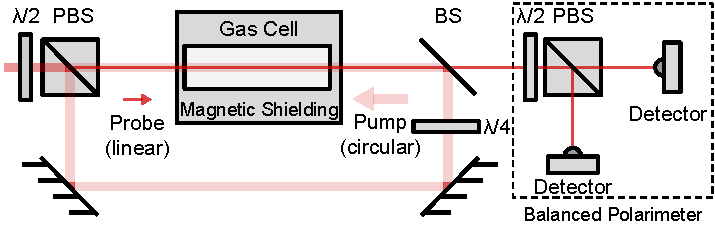
\includegraphics[width=\linewidth]{chapter1/Figs/PolSpecSchematic.pdf}
\caption{A schematic of \gls{ps} with a balanced polarimeter. The power balance between the probe and the pump beam is controlled with the left-most $\lambda/2$ phase retarder and \gls{pbs}. The $\lambda/4$ retarder is adjusted to produce a circularly polarised pump beam. The non-polarising beamsplitter (BS) is used to counter-propagate the pump beam through the atomic sample without altering the polarisation of the circular pump or linear probe. The final $\lambda/2$ retarder, \gls{pbs} and the detectors form the balanced polarimeter that monitors the polarisation rotation of the probe.}
\label{figure:pol_spec_schematic}
\end{figure}

The circularly polarised pump beam induces cicular birefringence in the atomic sample by partially optically pumping the sample into one of the extreme hyperfine sublevels, $m_F=\pm F$, where $m_F$ labels the hyperfine sublevel and $F$ labels {\color{red}some quentum thingy.}
This partial optical pumping, referred to here as the anisotropy fo the medium, results in unequal absorption coefficients for each circular polarisation.
The linearly polarised probe beam can be decomposed into two equal and oppositely circularly polarised components which undergo different absorption such that when recombined after passing through the atomic sample the probe beam becomes elliptically polarised with an angle different to that of the original linear polarisation.
This process is depicted in Figure \ref{figure:pol_spec_explanation}.

\begin{figure}
\centering
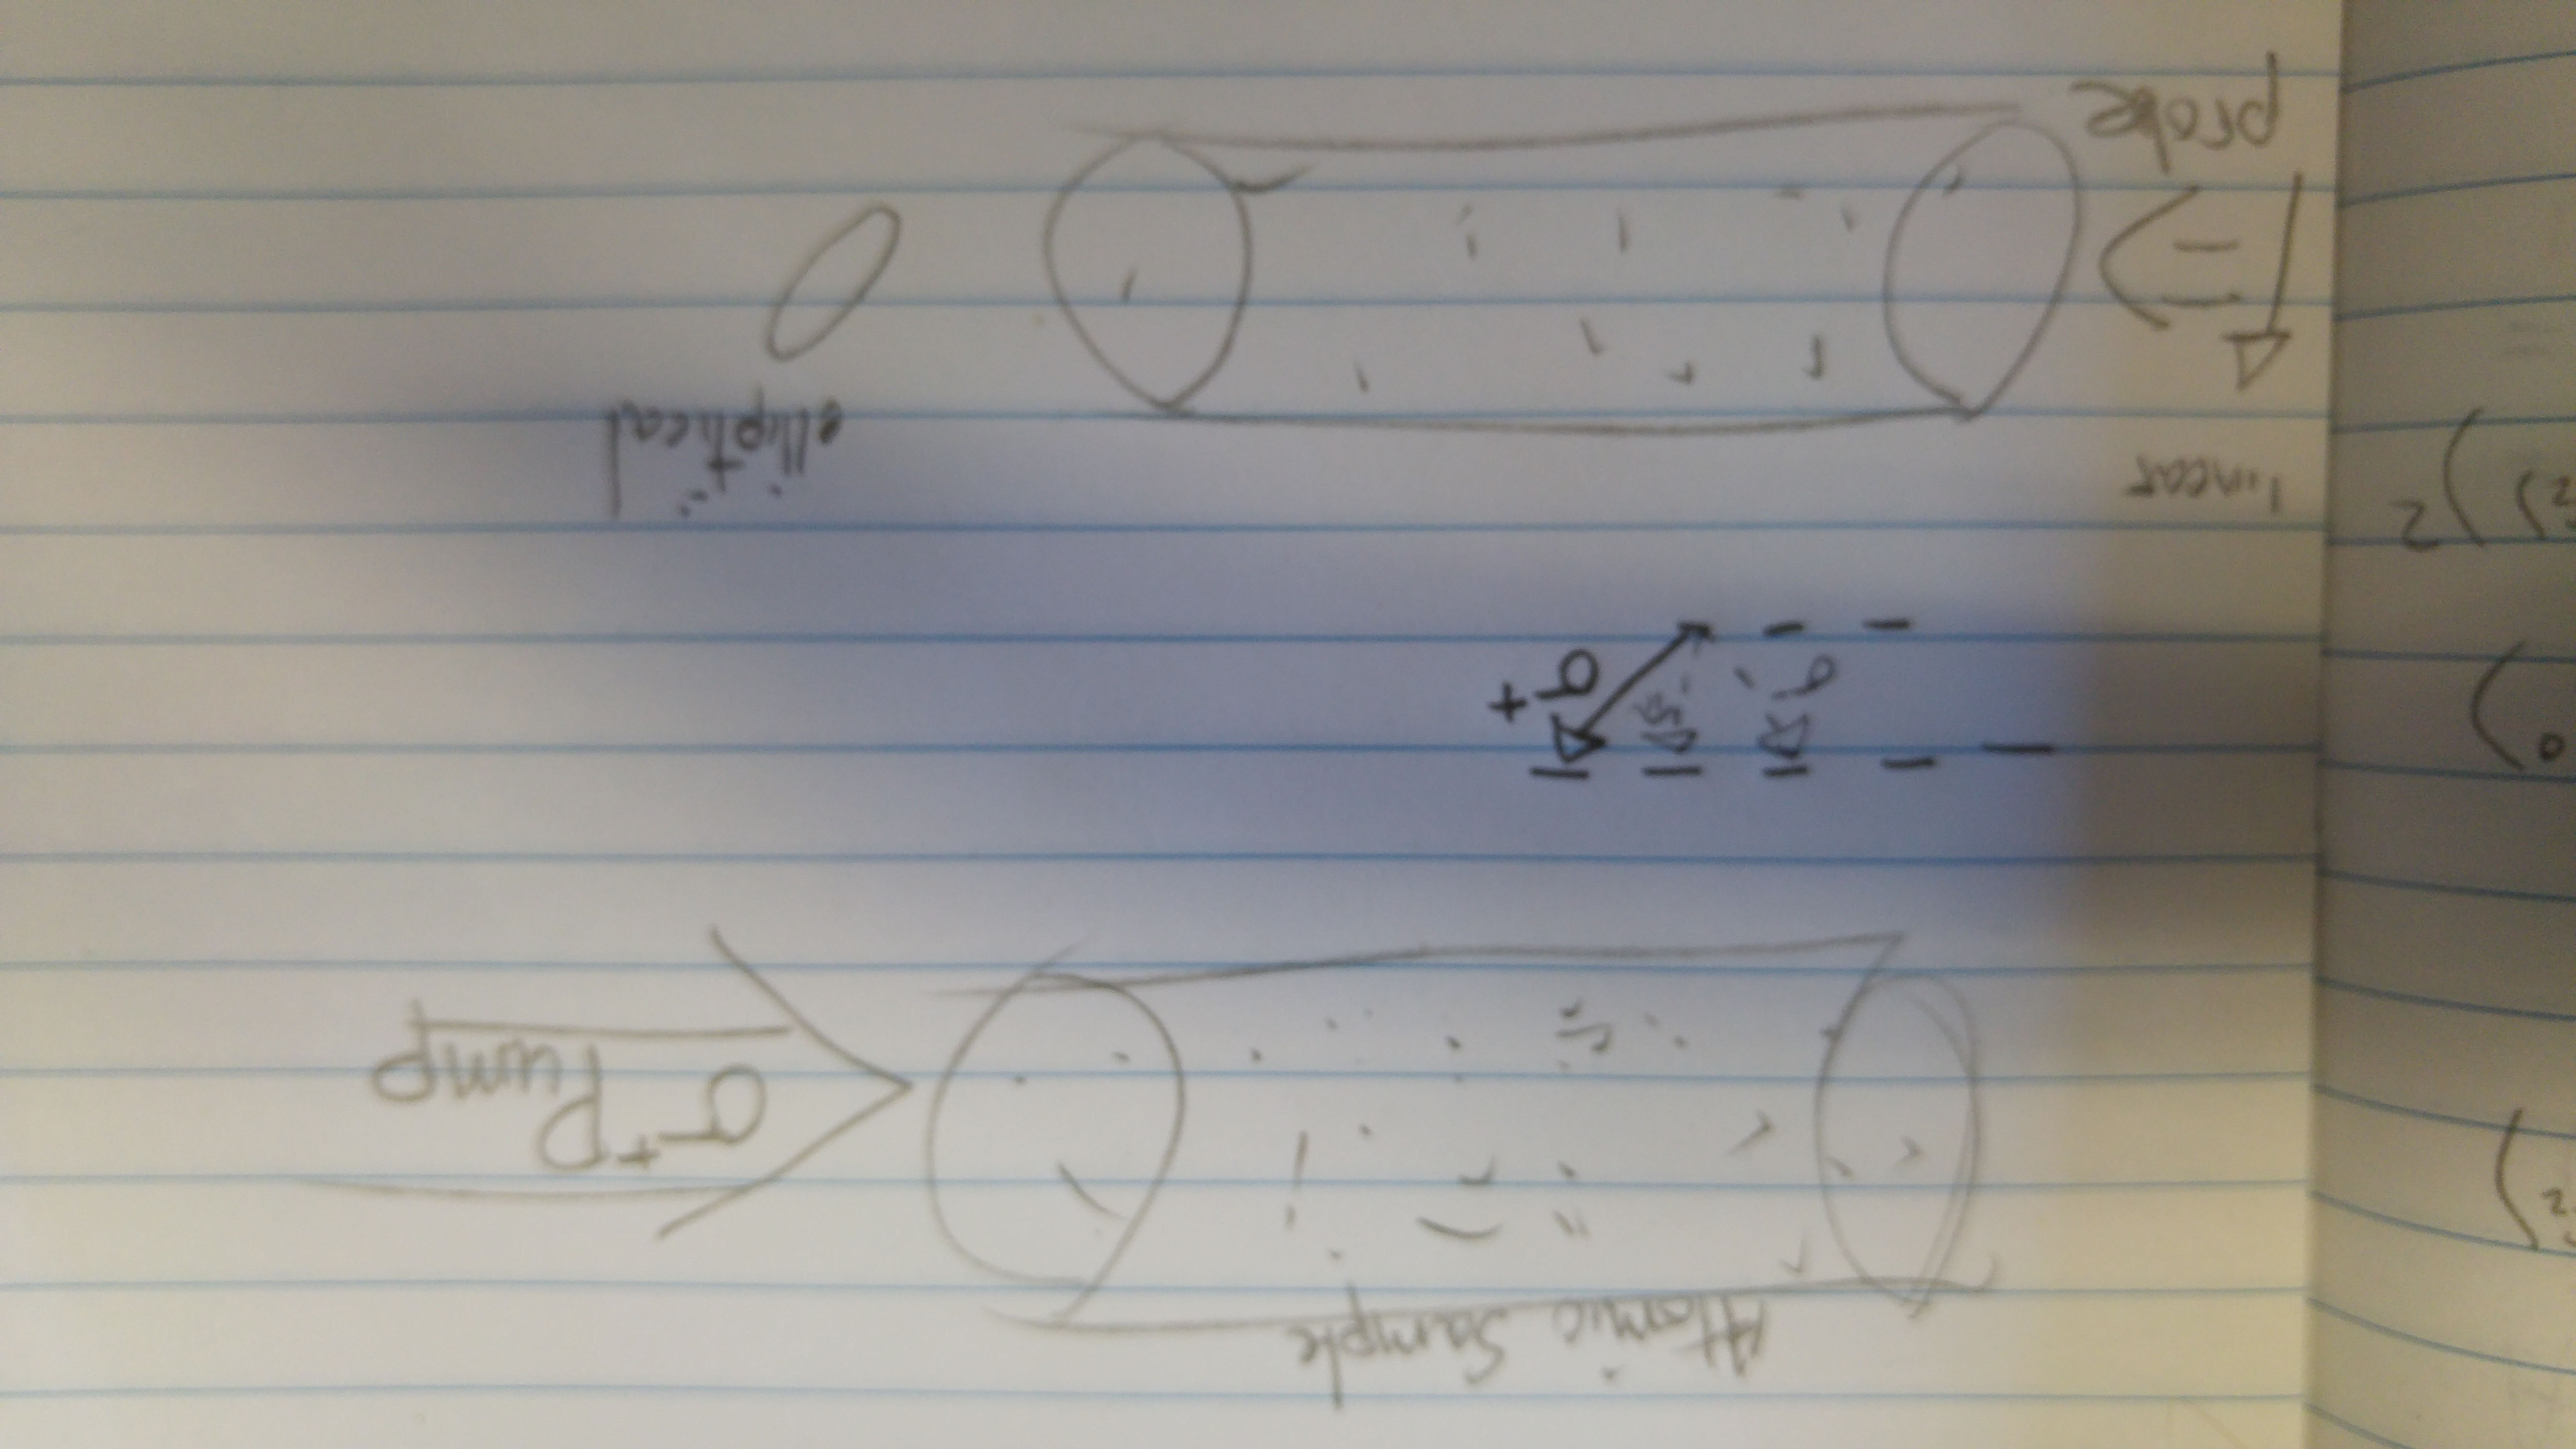
\includegraphics[width=\linewidth,angle=180]{chapter1/Figs/pol_spec_explanation_placeholder.jpg}
\caption{A conceptual figure for explaining the basics of pol spec.}
\label{figure:pol_spec_explanation}
\end{figure}


\subsubsection{Magnetic shielding}
\subsubsection{BS vs sneaking it past}
\subsubsection{Balanced polarimeter vs the other one}

\subsection{Fast Theory}
\subsection{OBEs (timescale of state evolution, step in simulating)}
\section{Developments}
\subsection{Balanced Polarimeter}
\subsection{Beam splitter to co-propagate}
\subsection{High bandwidth feedback}
\subsection{Lincoln's magic detectors?}
\section{Experimental Setup (with details - fibres, calcite, etc.)}
\section{Measurement Techniques}
\subsection{Self-heterodyne}
\subsection{Heterodyne}
\subsection{Noise measurements}
\subsection{Side of peak (include basic cavity theory here?)}
\subsection{Integration}
\subsection{Drift}
\subsection{Bandwidth Stuff}
